%------------------------------------------
%       $Id$
%
%       The GMT Documentation Project
%       Copyright (c) 2000-2013.
%       P. Wessel, W. H. F. Smith, R. Scharroo, J. Luis and F. Wobbe
%------------------------------------------
%
\chapter{Predefined bit and hachure patterns in \gmt}
\label{app:E}
\index{Attributes!fill!pattern}
\index{Fill!attributes!pattern}
\index{Pattern}

\GMT\ provides 90 different bit and hachure patterns that can be
selected with the \Opt{Gp} or \Opt{GP} option in most plotting programs.
The left side of each image was created using \Opt{Gp}, the right side
shows the inverted version using \Opt{GP}.
These patterns are reproduced below at 300 dpi using the default black and white shades.

\begin{center}
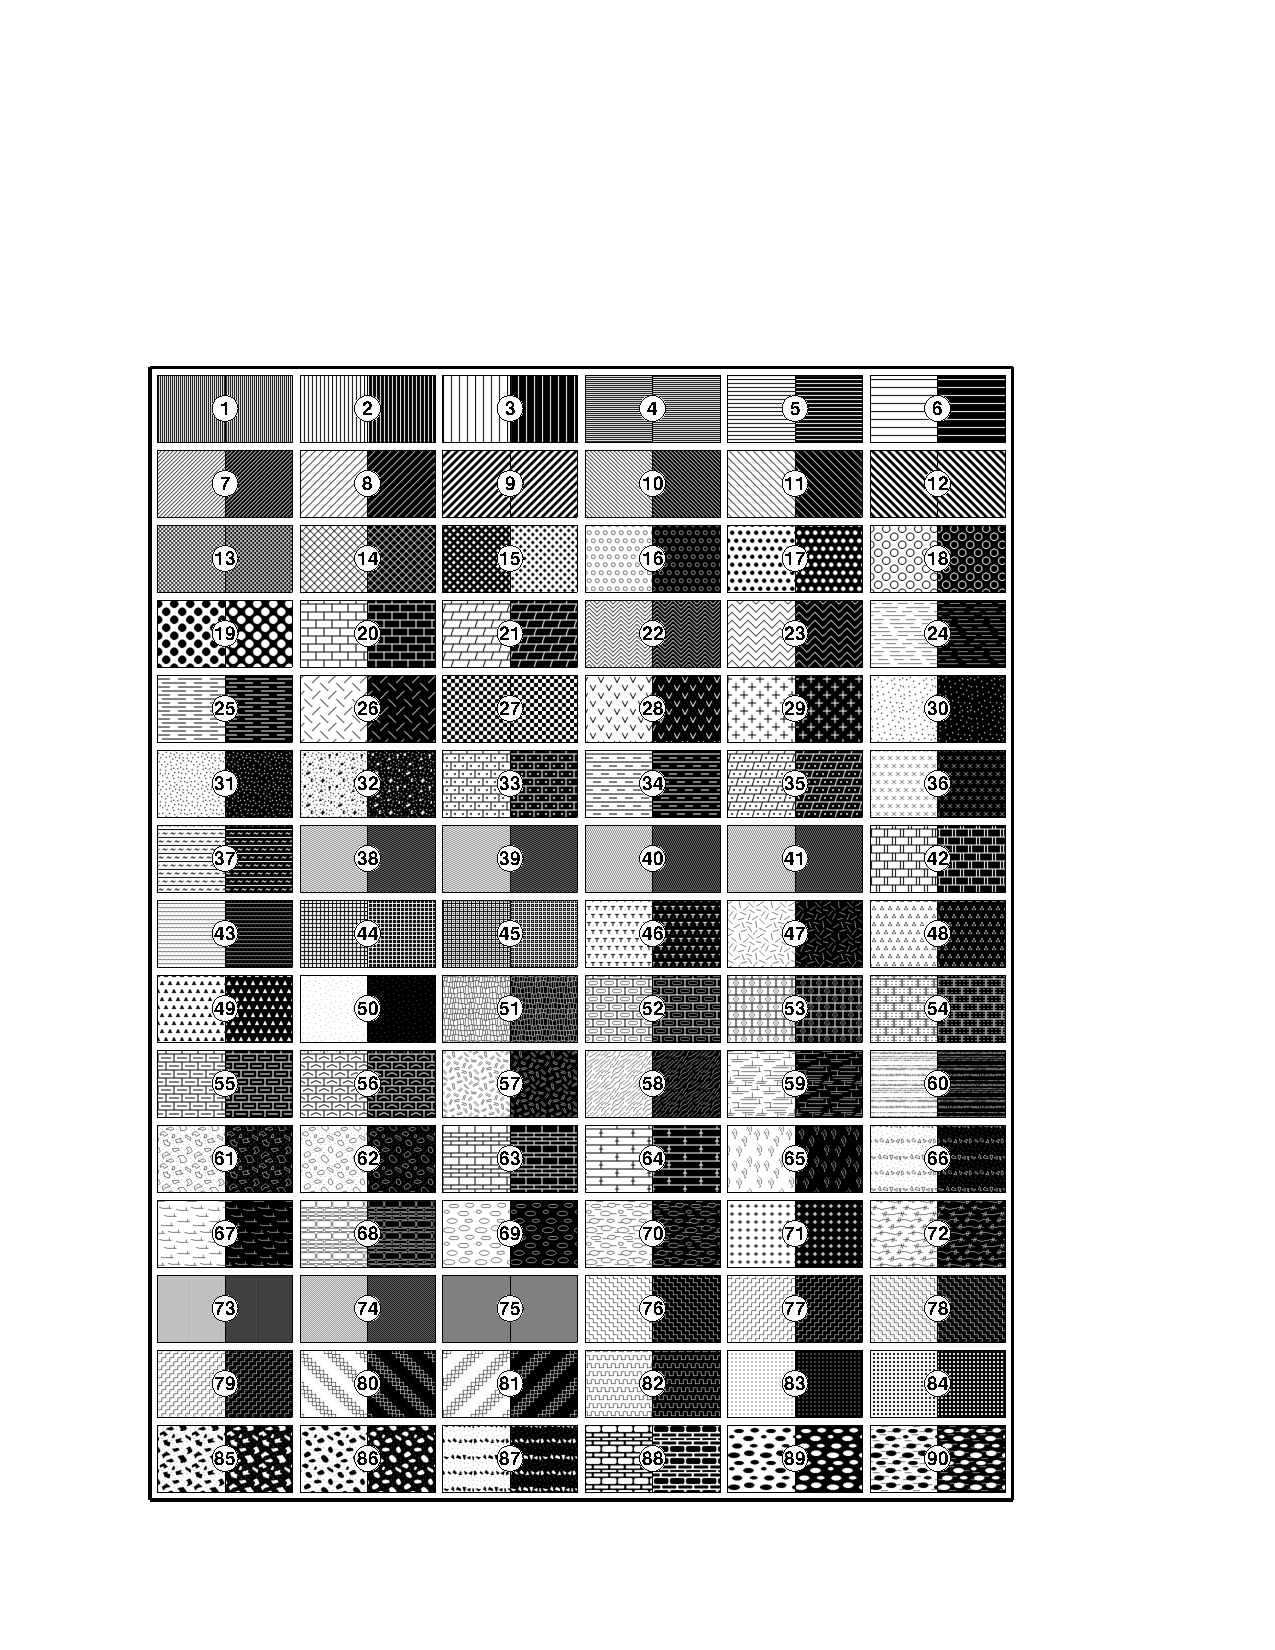
\includegraphics[scale=0.9]{GMT_App_E}
\end{center}
